\subsection{Actuator Control Attack}

This attack is implemented modifying the control algorithm inside the
\code{controller} FMU\@.

The attacker can choose some parameters:
\begin{itemize}
\item Real attack\_time: The time at which the attack starts.
\item Real attack\_duration: The duration, of the attack.
\end{itemize}

The objective of the attack is to set the input values for the actuators,
periodically, making the LFR go backward for an amount of time specified by
\code{attack\_duration} starting from \code{attack\_time}.

The control algorithm invoke the \code{actuator\_attack(State* st)} function at
the end of the code{tick(State* st)} function. 

\lstinputlisting[language=C, label={lst:actuatorattackcontrol},
caption={Actuator attack function.}]{actuator_attack_control.c}

\begin{figure}[htb]
	\centering
	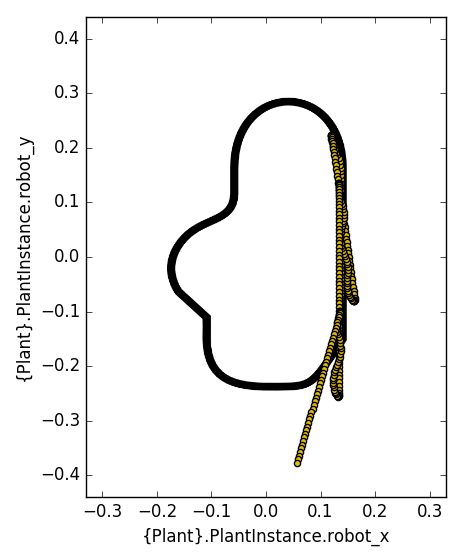
\includegraphics[width=0.5\textwidth]{img/actuator_attack_control.png}
	\caption{Line follower robot path when
	attacked}\label{fig:actuatorcontrolresult}
\end{figure}

In \figref{fig:actuatorcontrolresult} we can see the result of the attack: This
attack can be easily interpreted looking at the figures, the robot go forward
for a period of time and then it go backwards for \code{attack duration}
seconds.

